\section{Motivation}\labsec{ch01-motivation}

Each day more and more devices generate data both automatically and manually, and also each day the development of application in different domains that are backed by databases and expose these data to the web becomes easier. The amount and diversity of data produced clearly exceeds our capacity to consume it.

To describe the data that is so large and complex that traditional data processing applications can’t handle the term big data \sidecite[-100pt]{big-data} has emerged. Big data has been described by at least three words starting by V: volume, velocity, variety. Although volume and velocity are the most visible features, variety is a key concept which prevents data integration and generates lots of interoperability problems.

In order to solve this key concept RDF (Resource Description Framework) was proposed as a graph-based data model \sidecite[-150pt]{graph-data-model} which became part of the Semantic Web \sidecite[-125pt]{semantic-web} vision. Its reliance on the global nature of URIs\sidenote[][-100pt]{A Uniform Resource Identifier (URI) is a string of characters that unambiguously identifies a particular resource. To guarantee uniformity, all URIs follow a predefined set of syntax rules, but also maintain extensibility through a separately defined hierarchical naming scheme.\\Ref.\url{https://en.wikipedia.org/wiki/Uniform_Resource_Identifier}} offered a solution to the data integration problem as RDF datasets produced by different means can seamlessly be integrated with other data.

Also, and related to his is the concept of Linked Data \sidecite{linked-data} that was proposed as a set of best practices to publish data on the Web. It was introduced by Tim Berners-Lee and was based on four main principles:

\begin{itemize}
  \item Use URIs as names for things.
  \item Use HTTP URIs so that people can look up those names.
  \item When someone looks up a URI, provide useful information, using the standards (RDF, SPARQL).
  \item Include links to other URIs. so that they can discover more things.
\end{itemize}

\begin{marginfigure}
	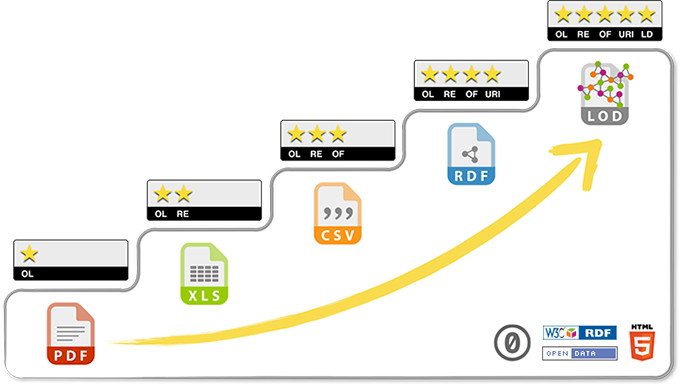
\includegraphics{5-star-steps}
	\caption[The 5 star steps of Linked Data]{The 5 star steps of Linked Data.}
	\labfig{margin-5-star-steps}
\end{marginfigure}

This four principles are called the 5 stars Linked Open Data Model, illustrated in \reffig{margin-5-star-steps}.
RDF is mentioned in the third principle as one of the standards that provides useful information. The goal of this principles is that data is not only ready for humans to navigate through but also for other agents, like computers, that may automatically process that data.

All the above motivations helped to make RDF the language for the Web of Data, as described in \sidecite{labra-validating-rdf}. And the main features that it presents are: Disambiguation, Integration, Extensibility, Flexibility and Open by Default. All this concepts will be deeply explored in \refsec{ch02-rdf}, but with the features also some drawbacks are associated, the most important one and the one we will focus is the RDF production/consumption dilema.

RDF production/consumption dilema states that it is necessary to find ways that data producers can generate their data so it can be handled by potential consumers. For example, they may want to declare that some nodes have some properties with some specific values. Data consumers need to know that structure to develop applications to consume the data.

Although RDF is a very flexible schema-less language, enterprise and industrial applications may require an extra level of validation before processing for several reasons like security, performance, etc.

To solve that dilema and as an alternative to expecting the data to have some structure without validation, Shape Expressions (ShEx) where proposed as a human-readable and high-level open source language for RDF validation. Initially ShEx was proposed as a human-readable syntax for OSLC Resource Shapes \sidecite{oslc-resource-shape} but ShEx grew very fast to embrace more complex user requirements coming from clinical and library use cases.

Another technology, SPIN, was used for RDF validation, principally in TopQuadrant’s TopBraid Composer. This technology, influenced from OSLC Resource Shapes as well, evolved into both a private implementation and open source definition of the Shapes Constraint Language (SHACL), which was adopted by the W3C Data Shapes Working Group.

From a user point of view the possibilities of ShEx are very large, from the smallest case to just validate a node with one property to a scientific domain case where we need to validate the human genome (a real use case of ShEx). As seen, ShEx is a new powerful language, but it can became complicated on the corner cases, but most of day-to-day uses can be solved with a subset of the language. This is the point where this project borns. We will call this subset ShEx-Lite. The simplicity of ShEx-Lite is not only focus on computer scientists who have experience the pain of new languages but also for other non-technical profiles that need to validate RDF data.

Besides to this, a common problem is that some companies use ShEx to define the constraints of the RDF data that they own. But then, when developing applications with object oriented languages they need to translate those schemas in to a domain model to support their data. Furthermore if the Shape Expressions used to validate their data changes for some reason they need to rewrite that domain model in the OOL again.

Finally, from a ShEx developer point of view sometimes appears the need to try new features in a small playground that allow easy an fast testing.
